%
% Diploma Thesis of Martin Kühl
% =============================
%
% Copyright (c) 2010  Martin Kühl <purl.org/net/mkhl>
%

%!TEX TS-program = xelatex
%!TEX encoding = UTF-8 Unicode

% Prelude
% =======
% (fold)

% Default Packages
% ----------------
\documentclass[11pt]{article}
\usepackage[a4paper]{geometry}
\usepackage{graphicx}
\usepackage{longtable}
\usepackage{float}
\usepackage{wrapfig}
\usepackage{soul}
\usepackage{alltt}
\usepackage{listings}
\usepackage{tocbibind}
\usepackage{textcomp}
\usepackage{marvosym}
\usepackage{wasysym}
\usepackage{latexsym}
\usepackage{amssymb}
\usepackage[parfill]{parskip}
\tolerance=1000

% Fancy Headings
% --------------
\usepackage{fancyhdr}
\pagestyle{fancy}
\lhead{}
\rhead{\itshape\leftmark\/}
\renewcommand{\sectionmark}[1]{\markboth{\thesection{}\hspace{1em}#1}{}}
\setlength{\headheight}{15pt}

% PDF Features
% ------------
\usepackage[
  xetex,
  unicode,
  pdfencoding=auto,
  pdftitle={Integrating Maude into Hets},
  pdfauthor={Martin Kühl},
  citecolor=blue,
  filecolor=black,
  linkcolor=blue,
  urlcolor=blue,
  bookmarks,
  breaklinks,
  colorlinks
]{hyperref}

% LaTeX Fonts
% -----------
% \usepackage{fixltx2e}
% \usepackage[utf8]{inputenc}
% \usepackage[T1]{fontenc}
% \usepackage{t1enc}
% \usepackage{lmodern}
% \usepackage{inconsolata}

% XeTeX Fonts
% -----------
\usepackage{mathspec, xltxtra, xunicode}
\defaultfontfeatures{Mapping=tex-text}
\setmainfont{TeX Gyre Pagella}
\setmathfont(Digits,Latin,Greek){TeX Gyre Termes}
\setsansfont{TeX Gyre Heros}
\setmonofont{TeX Gyre Cursor}

% Custom Commands
% ---------------
\newcommand{\Casl}{\textsc{Casl}}
\newcommand{\HetCasl}{\textsc{HetCasl}}
\newcommand{\Hets}{\textsc{Hets}}
\newcommand{\Spass}{\textsc{Spass}}
% Hets
\usepackage{hetcasl}
% Haskell
\lstloadlanguages{Haskell}
\lstset{
  language=Haskell,
  basicstyle=\small\ttfamily,
  commentstyle=\rmfamily\lstset{flexiblecolumns=true},
  basewidth={0.5em,0.45em},
  showstringspaces=false,
  numbers=left,
  firstnumber=1,
  stepnumber=10,
  numberfirstline=true,
  numberstyle=\footnotesize,
  % breaklines=true,
  % breakatwhitespace=true,
  literate=*{+}{{$+$}}1 {/}{{$/$}}1 {*}{{$*$}}1 {=}{{$=$}}1
            {>}{{$>$}}1 {<}{{$<$}}1 {\\}{{$\lambda$}}1
            {\\\\}{{\char`\\\char`\\}}1
            {->}{{$\rightarrow$}}2 {>=}{{$\geq$}}2 {<-}{{$\leftarrow$}}2
            {<=}{{$\leq$}}2 {=>}{{$\Rightarrow$}}2 {/=}{{$\neq$}}2
            {\ .}{{$\circ$}}2 {\ .\ }{{$\circ$}}2
            {>>}{{>>}}2 {>>=}{{>>=}}2
            {|}{{$\mid$}}1,
  literate={(c)}{{\copyright}}3 {$Header$}{{\textsc{Header}}}8
}


\date{August 16, 2010}

% (end)

% Content
% =======
\begin{document}

% Top Matter
% ----------
% (fold)
\begin{titlepage}
  \begin{minipage}{0.5\textwidth}
    \begin{flushleft}
      \begin{minipage}{6em}
        
\includegraphics[height=5em]{logo-uni.png}
      \end{minipage}
      \begin{minipage}{11em}
        \sffamily{\Large{}University\\ of Bremen\\}
      \end{minipage}
    \end{flushleft}
  \end{minipage}
  \begin{minipage}{0.5\textwidth}
    \begin{flushright}
      \begin{minipage}{6em}
        
\includegraphics[height=5em]{logo-fb3.png}
      \end{minipage}
      \begin{minipage}{11em}
        \sffamily{\Large{}Faculty 3:\\ Mathematics \&\\ Computer Science}
      \end{minipage}
    \end{flushright}
  \end{minipage}
  \vspace{5cm}
  \begin{center}
    \pdfbookmark[1]{Titlepage}{title}
    
    {\Large{}Diploma Thesis}
    
    \textbf{\Huge{}Integrating Maude into \Hets{}}
    
    \vspace{2cm}
    \textbf{\Large{}\href{http://purl.org/net/mkhl}{Martin Kühl}}\\
    {\large{}
     Matriculation Number: 1550788\\
     \href{mailto:mkhl@informatik.uni-bremen.de}%
          {mkhl@informatik.uni-bremen.de}}
    
    \vspace{2cm}
    {\Large{}
     Supervised by\\
     {\href{http://www.informatik.uni-bremen.de/~till/}%
           {Till~Mossakowski}}\\
     {\href{http://www.informatik.uni-bremen.de/theorie/kreo/}%
           {Hans-Jörg~Kreowski}}\\
    }
    
    \vfill
    {\large{}August 16, 2010}
  \end{center}
\end{titlepage}
\pagenumbering{Roman}
\pagestyle{empty}

\cleardoublepage

\begin{titlepage}
  \vspace*{0.5\textheight}
  I hereby confirm that I independently worked on and wrote this thesis and that I used only the references and auxiliary means indicated herein.

  \vfill
  \begin{flushright}
    \begin{minipage}{0.4\textwidth}
      Bremen, August 16, 2010

      \vspace{2cm}
      \rule{\textwidth}{0.5pt}
      \begin{center}
        Martin Kühl
      \end{center}
    \end{minipage}
  \end{flushright}
\end{titlepage}

\cleardoublepage
\pagenumbering{arabic}
\pagestyle{plain}

\tableofcontents

\pagebreak
\pagestyle{fancy}

% titlepage (end)

\clearpage
\section{Introduction} % (fold)
\label{sec:introduction}

\subsection{\Hets{} --- the Heterogeneous Tool Set}
\label{sub:introduction_hets}

\Hets{}~\cite{Mossakowski:2007} is a ``parsing, static analysis and proof management tool combining various tools for different specification languages''. On the practical level, it provides a framework for translating and integrating specification languages, logic implementations and proof management tools, based on a formalised system of institutions and institution comorphisms.

Providing this form of integration, \Hets{} can be considered as similar to a motherboard~\cite{Codescu:2010} ``where different expansion cards can be plugged in, the expansion cards here being individual logics (with their analysis and proof tools) as well as logic translations''. Each additional expansion supplements the framework as a whole and lets users choose a more suitable and flexible set of tools to handle their specification and proof management needs.

The core of \Hets{} operates independently from concrete logics and organises specifications in development graphs~\cite{Mossakowski:2006a}, where nodes are used to represent theories, annotated with their respective logic systems, and edges denote dependencies between the theories, corresponding to the structuring mechanisms of the language \Casl{}~\cite{Astesiano:2002}. Concrete logics are represented by institutions~\cite{Mossakowski:2005a}, an abstract formalisation of the notion of a logic system. The logic transformations currently supported by \Hets{} can be found in~\cite{Mossakowski:2006b}.


\subsubsection{Example: \Hets{}}
\label{sub:introduction_hets_example}

Figure~\ref{ex:casl-spo} contains a simple \Casl{} specification of a strict partial order and a partial order, the latter being defined in terms of the former and the built-in notion of equality. It then declares that reflexivity, antisymmetry  and transitivity of the partial order can be derived from this definition.

\begin{figure}
  \input{SPO_PO.pp.tex}
  \caption{Example \Casl{} Specification}\label{ex:casl-spo}
\end{figure}

Feeding this example to \Hets{} generates the development graph displayed in Figure~\ref{fig:casl-spo-before}. Note the link from \textsc{Partial\_Order} back to the unlabelled node.\footnote{With coloured output, it would be displayed in red.} This link represents the proof obligations introduced by the \emph{implied extension} of the \textsc{Partial\_Order} theory.\footnote{Implied extensions are defined with the \textbf{then \%implies} syntax.~\cite{Mosses:2004}} Once the properties in question have been proven in a way integrated with \Hets{}, the graph is modified to look like in Figure~\ref{fig:casl-spo-after}; the proof obligations have been discharged and their target node is either redisplayed\footnote{With coloured output, they are also displayed in green.} or, as in this example, subsumed into its originating theory.

\begin{figure}
  \begin{minipage}[b]{0.5\textwidth}
    \begin{centering}
	    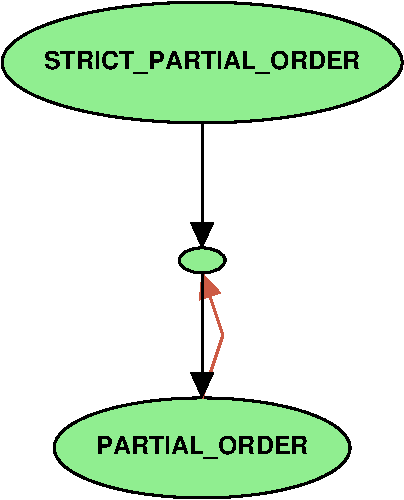
\includegraphics[width=7cm]{SPO_before.pdf}
	    \caption{Open Proof Obligations}\label{fig:casl-spo-before}
    \end{centering}
  \end{minipage}
  \begin{minipage}[b]{0.5\textwidth}
    \begin{centering}
	    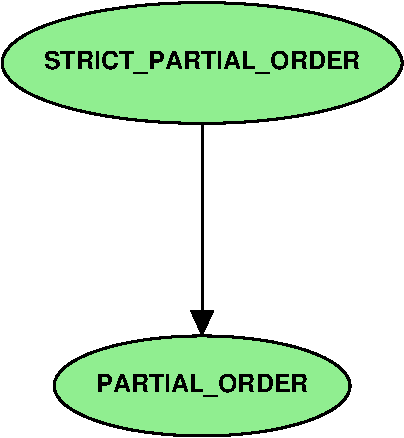
\includegraphics[width=7cm]{SPO_after.pdf}
	    \caption{Proof Obligations Discharged}\label{fig:casl-spo-after}
    \end{centering}
  \end{minipage}
\end{figure}

Discharging proof obligations with \Hets{} is done by moving them to a node, usually with the command \emph{Proofs$\rhd$Automatic}, and selecting the \emph{Prove} command on that node, which displays the dialogue in Figure~\ref{fig:casl-spo-prove}. Here we can inspect our axioms and proof goals and launch a theorem prover to work on the goals using the axioms. For more information on interacting with \Hets{}, refer to~\cite{Mossakowski:2006b}.

In this case, the goals are simple enough to be proven with \Spass{}~\cite{Weidenbach:2009}, an automated theorem prover for first-order logic with equality, with which we can interact through the dialogue in Figure~\ref{fig:casl-spo-spass}. More complex proofs are usually performed with Isabelle\cite{Nipkow:2002}, an advanced interactive proof assistant for higher-order logic.\footnote{Not displayed. Interaction with Isabelle is usually via an Emacs instance.}

\begin{figure}
  \begin{minipage}[b]{0.5\textwidth}
    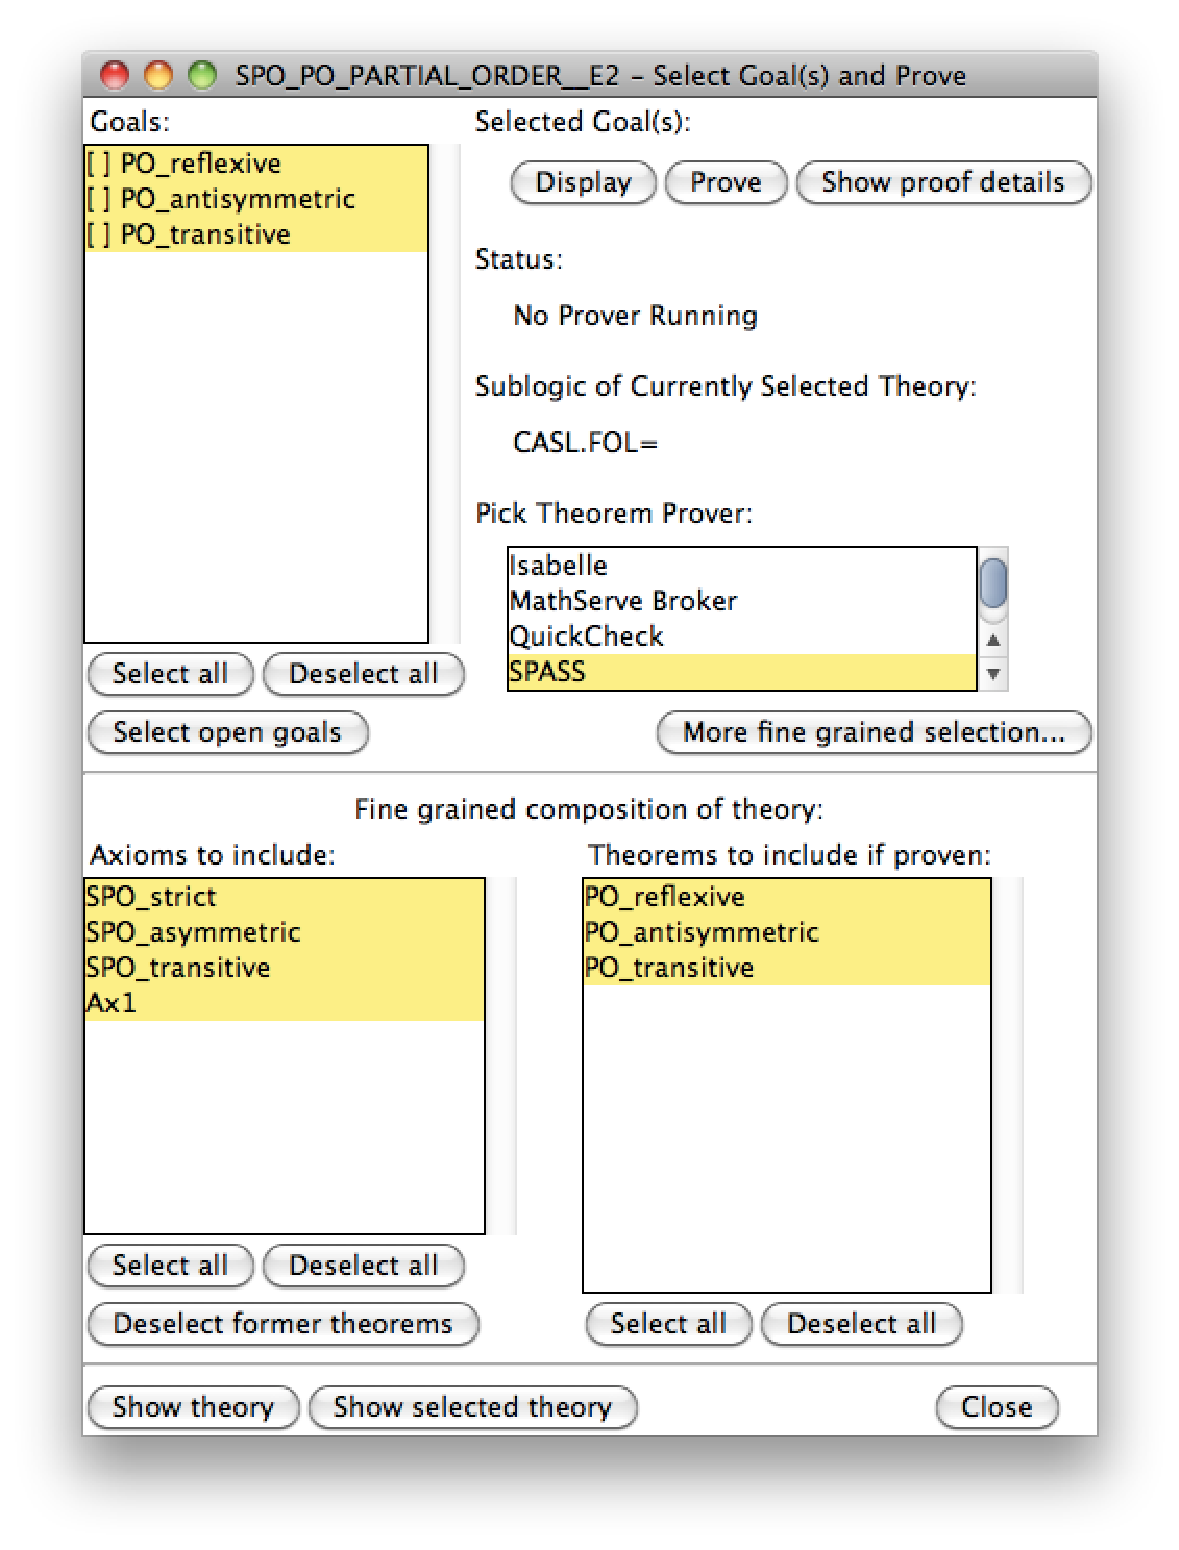
\includegraphics[width=\textwidth]{SPO_prove.pdf}
    \caption{Proving Theorems in \Hets{}}\label{fig:casl-spo-prove}
  \end{minipage}
  \begin{minipage}[b]{0.5\textwidth}
    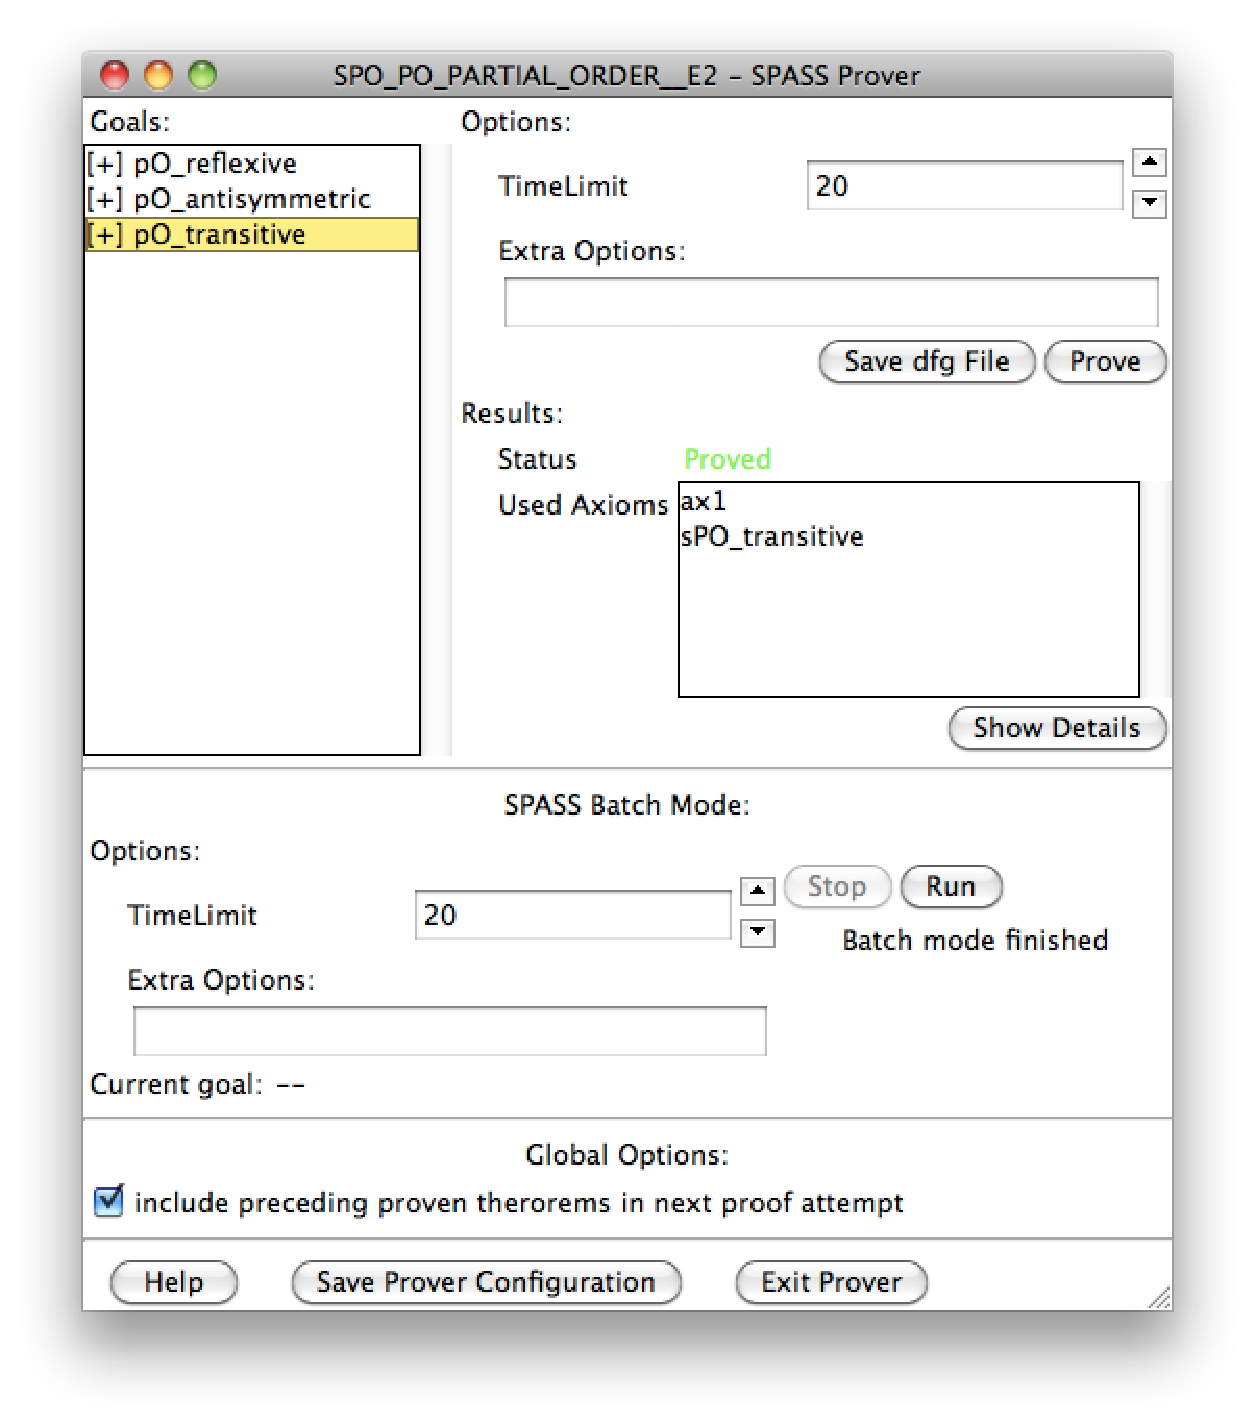
\includegraphics[width=\textwidth]{SPO_spass.pdf}
    \caption{Successful Proof with \Spass{}}\label{fig:casl-spo-spass}
  \end{minipage}
\end{figure}


\subsection{Maude --- a Rewriting Logic Computation System}
\label{sub:introduction_maude}

Maude~\cite{Clavel:2003} is a ``high-performance reflective language and system supporting both equational and rewriting logic specification and programming for a wide range of applications''. Maude is described as based on rewriting logic~\cite{Meseguer:1992}, ``a logic of actions whose models are concurrent systems'' that is ``sound and complete and has initial models''.

The core of Maude is based on equational algebra, strongly influenced by the OBJ3 language~\cite{Goguen:1993,Clavel:2002}, while its additional support for rewriting logic computation makes Maude particularly well suited for modelling concurrent, distributed and object-oriented systems. Maude also features powerful reflective capabilities and is able to fully metarepresent itself. A variant of Maude called \emph{Full Maude}~\cite{Duran:1999} has even been implemented completely in Maude.

With its high performance and expressive and flexible syntax, Maude is a viable choice as a programming language as well as a specification language. Its rigorous mathematical foundation makes Maude suitable for implementing logical languages and providing them with executable semantics. A system with Maude's capacity for reflection is also an obvious target for tool support.

It should be noted that Maude was recently discovered~\cite{Codescu:2010} to not actually be based on rewriting logic as defined in~\cite{Meseguer:1992}. The conclusion is that preordered algebra~\cite{CafeObjRep} should be used for Maude, the essential difference being that rewrite rules are no longer labelled or even distinguished. Refer to~\cite{Codescu:2010} for details on the specific differences.


\subsubsection{Example: Maude}
\label{sub:introduction_maude_example}

In Figure~\ref{ex:maude-natlist} we demonstrate using Maude to specify lists of natural numbers. We begin by defining a module \textsc{NatList} to contain the specification, in this case a \emph{functional module} (\texttt{fmod}) because we only use equational simplification; rewriting rules are available in \emph{system modules} (\texttt{mod}). Natural numbers and their sort $Nat$ are predefined in the \textsc{Nat} module, which we import in \emph{protecting} mode\footnote{For more about importation modes, see~\cite[ch. 8.1]{Clavel:2007}.}. This also provides the common decimal notation for numbers as well as the usual operations.

Next we declare a sort $NatList$, representing lists of natural numbers, and $Nat$ as a subsort of $NatList$ so we can treat numbers as singleton lists. As constructor terms for lists we define the empty list $nil$ and a concatenation operator, denoted here with an infix comma\footnote{The underscores determine the positions of parameters.}, followed by two additional operators $len$ (length) and $rev$ (reverse). The rules for simplifying these operators correspond to their obvious respective inductive definitions and are defined in the remainder of the listing.

The Maude system defines executable semantics for languages specified with it, and can be used to interactively examine its properties. Figure~\ref{tr:maude-natlist} shows a transcript of such a session\footnote{\texttt{Maude>} is the prompt of the interactive system.} for the module described above. First we demonstrate use of the \texttt{parse} command to parse and type-check terms. Notice that operator properties other than their type, like $nil$ being the identity for concatenation, are not considered at this level, and that no simplification or rewriting is attempted.

Next we use \texttt{reduce} to simplify terms and perform calculations. Maude applies equational simplifications until it arrives at a \emph{canonical} term to which no further rules apply. To also consider rewriting rules requires using the \texttt{rewrite} command instead. The \texttt{match} command, finally, provides a simple interface to Maude's pattern matcher. Note that this command operates purely syntactically, i.e.\ no simplification is attempted to match the terms.

\begin{figure}
  \begin{minipage}[b]{0.5\textwidth}
    \begin{alltt}\footnotesize{}\input{NatList.maude}\end{alltt}
    \caption{Example Maude Module}\label{ex:maude-natlist}
  \end{minipage}
  \hspace{2.5mm}
  \begin{minipage}[b]{0.45\textwidth}
    \begin{alltt}\footnotesize{}\input{NatList.typescript}\end{alltt}
    \caption{Example Maude Interaction}\label{tr:maude-natlist}
  \end{minipage}
\end{figure}


\subsection{Motivation and Overview}
\label{sub:introduction_overview}

The general benefits of integrating any system into \Hets{} are obvious: Having more languages and logic systems available to write specifications in, more tools to work with on these specifications, we can enable users familiar with a newly integrated system to work with \Hets{} and make use of its proof management facilities. They could, for example, use \Hets{} and its tools to formally verify existing specifications written with their familiar system.

There are additional reasons to specifically integrate Maude as well: Maude is a robust and highly performant rewriting engine, that easily enables the execution of systems defined with it --- or translated into it. This facilitates an interactive style of specification development with a short feedback loop between user and machine, and provides ways to explore and examine the specified system as demonstrated above in section~\ref{sub:introduction_maude_example}.

Mosses also notes in~\cite{Mosses:2008} that Maude and its underlying logic are well suited for working with object-orientation or concurrency, and that this capability is not present in \Casl{} or other languages supported by \HetCasl{} at this time. Adding it would help make \Hets{} more applicable to this problem domain.

The rest of this document is organised as follows:
\begin{description}
  \item[Section~\ref{sec:analysis}] examines ways and options for integrating Maude with \Hets{} and sets goals for the strategy and extent of integration described in this work.
  \item[Section~\ref{sec:implementation}] describes the implementation that realises this integration.
  \item[Section~\ref{sec:results}] discusses the results of the integration and illustrates them with examples.
  \item[Section~\ref{sec:conclusion}] concludes and outlines future work.
  \item[Appendix~\ref{sec:appendix_implementation}] contains listings of the Haskell modules this work resulted in.
  \item[Appendix~\ref{sec:appendix_example}] presents additional examples.
\end{description}

% section introduction (end)

\clearpage
\section{Analysis} % (fold)
\label{sec:analysis}

\Hets{} and Maude are both large systems consisting of many parts; integrating both can be done in different ways, targeting different components, and supporting different feature sets. In particular, we need to determine how to fit Maude into \Hets{} concepts of logics and tools, and to which extent to support the Maude language.

This section explores the space of options for integrating Maude into \Hets{} and defines the goals for this work.

\subsection{Integration Options}
\label{sec:2_1}

\subsubsection{Maude Institution}
\label{sec:2_1_1}

Maude is a logic system; in order to relate new logics with those supported by \Hets{}, we need to formulate them in terms of its formal framework, i.e.\ as an institution. An institution consists of a category of signatures and signature morphisms, classes of sentences and models, and an entailment relation that is stable under signature morphism.

The full definition of the institution $Maude^{pre}$, based on Maude's preordered algebra semantics, can be found in~\cite{Codescu:2010}; its signature category is briefly summarised here:

\begin{itemize}
  \item \emph{Signatures} are tuples $(K, F, kind : (S, \leq) \rightarrow K)$, where $K$ is a set of kinds, $kind$ a function assigning to each sort in $(S, \leq)$ a kind, and $F$ a set of function symbols along with their arity.
  \item \emph{Signature morphisms} are functions $\Phi$ over signatures, with component functions $\Phi^{kind}$ mapping kinds and preserving subsorting, $\Phi^{sort}$ mapping sorts such that subsorting is preserved and $kind$ assignment commutes with $\Phi^{kind}$, and $\Phi^{op}$ mapping function symbols compatibly with type mappings and preserving overloading.
  \item \emph{Sentences} of a signature $\Sigma$ are Horn clauses whose atoms are equational $t = t'$, membership $t : s$ or rewrite atoms $t \Rightarrow t'$, where $t, t'$ are $F$-terms and $s$ is a sort in $S$.
\end{itemize}

The definitions of models and the entailment relation is not directly relevant to this work; refer to~\cite{Codescu:2010} for details.


\subsubsection{Translation Maude $\rightarrow$ \Casl{}}
\label{sec:2_1_2}

A logic translation from Maude to \Casl{}, formalised as an institution comorphism and corresponding to an encoding of Maude in \Casl{}, would allow \Hets{} to accept Maude specifications as input and handle them by translating them to \Casl{}\footnote{And from there to other supported languages.} before passing them on to theorem provers.

We use \Casl{} because the language is well-supported and -understood and plays a central role in \Hets{}, providing the structuring mechanisms used in its development graphs.

This form of integration depends on the definition of a logic translation for Maude as per section~\ref{sec:2_1_1}. It would allow users to specify systems\footnote{Or parts of systems.} in Maude and verify them with any tool supported by \Hets{}. The proof obligations introduced by Maude views\footnote{See also section~\ref{sub:results_proof_goals} and~\cite[ch. 6]{Clavel:2007}}, for example, can be formally verified with \Hets{}; Maude itself does not provide any support for this.

This is the form we chose to implement. It essentially adds support for an additional input language to \Hets{}, including all its motivating features mentioned in Section~\ref{sub:introduction_overview}, while also making the whole \Hets{} infrastructure available for Maude specifications.


\subsubsection{Translation \Casl{} $\rightarrow$ Maude}
\label{sec:2_1_3}

Complementary to the translation described in Section~\ref{sec:2_1_2}, this one corresponds to encoding \Casl{} in Maude. It would allow \Hets{} to translate any specification to Maude if it can be translated into \Casl{}, which is the case for most languages in \Hets{}.

Provided with this form of integration, users could specify systems in \Hets{} with any of its languages and at any point translate the specifications into Maude, then use Maude and its related tools to work on the specification, allowing the use of Maude's rewriting capabilities on \Casl{} equations. The downside is that \Hets{} would not be aware of the results so they could not be fed back into the development graph. This form also requires the logic translation for Maude from section~\ref{sec:2_1_1} to be defined.

This form, adding multiple input languages for Maude and an additional tool with limited usage for \Hets{}, provides fewer benefits for \Hets{}. Support for concurrency or distributed specifications in \Hets{} would also be missing; we decided in favour of the complementary option.


\subsubsection{Maude Proof Assistant}
\label{sec:2_1_4}

Instead of as a logic system, Maude can be integrated into \Hets{} as a proof assistant tool. This way users could specify systems in \Hets{} and, from inside of \Hets{}, use Maude to examine, execute or verify them while still being able to use \Hets{}'s other tools on the same specification.

This approach requires some language, say \Casl{}, to be translated into Maude, which can either be done by defining the translation described in Section~\ref{sec:2_1_3} or by pragmatically implementing a syntactic transformation.

The latter option would lack the formal rigidity one can reasonably expect from tools in this domain, making it less appealing from a formal or mathematical perspective. The former has appeal but would have exceeded the time constraint on this work.


\subsection{Extent of the Integrated Language}
\label{sec:2_2}

\subsubsection{Core Maude vs.\ Full Maude}
\label{sec:2_2_1}

There are two languages sharing the name ``Maude'': \emph{Core Maude}~\cite{Clavel:2002}, with its interpreter implemented in C++, provides all basic functionality of Maude, including all features mentioned in Section~\ref{sub:introduction_maude} like syntax, module structure, reflection etc.; \emph{Full Maude} is an extension of Core Maude, written in Maude itself and available as a Core Maude module, which adds features like parametrised views\footnote{In Core Maude, only modules can be parametrised, not views.} and object-oriented modules, providing special notation for objects, messages, classes and inheritance.

While Full Maude features interesting properties, the fact that it is an extension of Core Maude implies that supporting the latter should be the first step when aiming to support the former. Full Maude is also more of a moving target, evolving faster than Maude due to its more high-level implementation language. For these reasons we chose to begin by integrating Core Maude into \Hets{} and leave the extension to Full Maude to future work.

In the sequel (and, in fact, the prequel) we use \emph{Maude} to refer to the \emph{Core Maude} implementation unless the distinction is either not obvious from context or meant to be emphasised.


\subsubsection{Functional Maude vs.\ System Maude}
\label{sec:2_2_2}

Another distinction within Maude can be made between functional modules and system modules~\cite{Clavel:2007}, which are just an extension of functional modules with rewrite rules. We can formalise this distinction by defining languages \emph{System Maude}, identical to Core Maude and allowing the use of system modules, and \emph{Functional Maude}, a subset of Core Maude restricted to functional modules.\footnote{The terminology here is introduced to illustrate a point and will not be reused.}

In a conclusion similar to that in Section~\ref{sec:2_2_1}, one may assume that this suggests limiting an integration to Functional Maude at first; rewrite rules and the properties specific to their underlying logic are, however, an integral part of the motivation to integrate Maude in the first place, so leaving them out would practically obsolete this work. Implementing them in parallel to the functional parts also makes sense from a pragmatic standpoint: Their later addition would require changes throughout the modules implementing support for Functional Maude, like views and renamings, to support their handling of rewrite rules; in contrast, the features needed for Full Maude, say object-oriented modules, are orthogonal to Core Maude.

From this we decided to implement support for all of Core Maude, not just a functional subset of it, but given the time pressure on this work, we would focus tests of the resulting integration on the functional parts and move on to the details of rewriting once those were satisfactory.


\subsection{Goals of This Work}
\label{sec:2_3}

In summary: Given the institution for Maude described in~\cite{Codescu:2010}, we will implement a translation from Maude to \Casl{} based on this institution. The translation will support all of Core Maude, including system modules, in a way such that Maude modules can be used in \Hets{}.

% section analysis (end)

\clearpage
\section{Implementation} % (fold)
\label{sec:implementation}

\subsection{The \texttt{Logic} Type Class}
\label{sub:implementation_logic_hets}

In order for a logic to be integrated with \Hets{}, its implementation must provide an \emph{identity type}, identifying it and implementing the type class \texttt{Language}, and a system of related data types implementing the type class \texttt{Logic}, defined in the \texttt{Logic.Logic} module. This class provides the abstract interface between concrete logics and the logic independent parts of \Hets{}.

These other types are required to define a logic:

\begin{description}
  \item[Symbols] identify sorts, predicates, operators, variables etc.,\ fully qualified with their symbol type.
  \item[Signatures] provide ``vocabularies'' of symbols to construct terms from, together with their complete typing information.
  \item[Sentences] are equivalent to logical formulae, constructed from terms in a way supported by the underlying logic.
  \item[Signature morphisms] (sometimes just called morphisms) define mappings between signatures, usually preserving their structure.
  \item[Basic Specifications] denote a signature together with a set of sentences, translated into abstract syntax.
\end{description}

Supported by these types, the logic is then required to define instances for the following type classes as illustrated by Figure~\ref{fig:logic-class-hierarchy}:

\begin{description}
  \item[\texttt{Language}] associates the logic with a human-readable name and description.
  \item[\texttt{Category}] defines a category of the logic's signatures and signature morphisms with the usual operations identity, composition, domain and codomain.
  \item[\texttt{Syntax}] provides facilities to parse and print abstract syntax, i.e.\ basic specifications as well as symbol lists and maps.
  \item[\texttt{Sentences}] relates symbols and sentences to a signature/morphism category and supplies ways to translate sentences along morphisms, extract symbol lists from signatures and symbol maps from morphisms, and pretty-print signatures and sentences.
  \item[\texttt{StaticAnalysis}] is used for (statically) analysing basic specifications, computing its axioms and signature. It also provides additional operations on signatures and morphisms like generating their unions, intersections, inclusions and empty instances.
  \item[\texttt{Logic}] is the central interface for logics in \Hets{}. Besides including the above classes, it adds a sublogic mechanism so related logics can share the implementations of logic-related classes.
\end{description}

\begin{figure}[htbp]
  \includegraphics[width=\textwidth]{logic-class-hierarchy.pdf}
  \caption{The class hierarchy of the \texttt{Logic} module}\label{fig:logic-class-hierarchy}
\end{figure}

The remainder of this section describes our implementation of the logic corresponding to Maude in Haskell, and its integration into \Hets{} via the \texttt{Logic} type class.


\subsection{Abstract Syntax of Maude}
\label{sub:implementation_abstract_syntax}

The abstract syntax of Maude is modelled after its formal grammar~\cite{Clavel:2007} and implemented in the module \texttt{Maude.AS\_Maude} in appendix~\ref{imp:Maude/AS_Maude.hs}. It represents specifications as Maude modules, theories and views. Each non-terminal of the grammar is translated into a Haskell data type while identifiers\footnote{Terminals are either identifiers or syntactic structure.} are summarily modelled by the \texttt{Qid} type (short for \emph{quoted identifier}). These identifiers are the atoms making up terms and statements which, in turn, constitute modules.

All abstract syntax types are instances of the type classes \texttt{Show}, \texttt{Read}, \texttt{Eq}, \texttt{Ord} and \texttt{Pretty}\footnote{\texttt{Pretty} is provided by \Hets{}, the rest by the Haskell 98 standard.} so they can trivially be pretty-printed and used in Haskell collection types. In fact, Maude modules are loaded by way of a Maude program parsing them and generating a string representation compatible with the \texttt{Read} instance of the corresponding abstract syntax class.


\subsection{Symbols}
\label{sub:implementation_symbols}

A symbol identifies a sort, kind, label or an operator. The \texttt{Symbol} type, from module \texttt{Maude.Symbol} in appendix~\ref{imp:Maude/Symbol.hs}, represents such an identifier, annotated with the information, which kind of symbol it identifies. Additionally, operators that are qualified with their arity are distinguished from those that explicitly match operators of arbitrary arity.

Common operations on symbols are conversion to other types of symbols, qualification with their containing module, extraction of their contained information, and testing inside a subsort relation, i.e.\ given a subsort relation, testing whether two symbols belong to the same kind.

Instances of \texttt{Show}, \texttt{Read}, \texttt{Eq}, \texttt{Ord} and \texttt{Pretty} are provided, and the module defines the types \texttt{SymbolSet} to be a set of symbols and \texttt{SymbolMap} to be a map taking symbols to symbols.


\subsection{Meta Operations}
\label{sub:implementation_meta}

Early on in the implementation phase it became apparent that the most commonly used component types would be names (i.e.\ qids) and symbols. The most frequently used operations associated with collections of these types are extraction of component data (e.g.\ the name of an operator or the set of sorts of a signature), modification of that data (e.g.\ renaming the sorts of a sentence), and conversion of data to symbols. These operations proved pervasive enough to warrant their implementation as Haskell type classes and corresponding instances for all supported types used in the Maude logic.

The simplest of these classes, called \texttt{HasName}, provides two operations:

\begin{description}
  \item[\texttt{getName}] extracts the name of the instance,
  \item[\texttt{mapName}] maps the name of the instance along a function.
\end{description}

The symbol types we are interested in for this purpose are sorts, labels and operators, in other words the ``named'' symbols.\footnote{Kinds are identified by the names of their associated sorts.} The corresponding type classes are called \texttt{HasSorts}, \texttt{HasLabels} and \texttt{HasOps} respectively; the operations of these classes, \texttt{getSorts} and \texttt{mapSorts} for \texttt{HasSorts}, analogously for the others, extract symbol sets from their instances and map their instances' components along symbol maps.

Finally, \texttt{AsSymbol} is instantiated by types that can be converted to symbols. Besides the obvious conversion function, which is called \texttt{asSymbol} if it is a total operations and \texttt{asSymbolMaybe} if it is partial, this class also provides utilities to (trivially) convert instances to symbol sets (\texttt{asSymbolSet}) and to transform an instance along a symbol map (\texttt{mapAsSymbol}) by converting it to a symbol and converting the mapped symbol back to the instance type.

The above classes are defined in eponymous modules under the \texttt{Maude.Meta} namespace, listed in appendices~\ref{imp:Maude/Meta/AsSymbol.hs}, \ref{imp:Maude/Meta/HasLabels.hs}, \ref{imp:Maude/Meta/HasName.hs}, \ref{imp:Maude/Meta/HasOps.hs} and~\ref{imp:Maude/Meta/HasSorts.hs}, and are summarily exported in the \texttt{Maude.Meta} module in appendix~\ref{imp:Maude/Meta.hs}. Default implementations of the classes are provided for the abstract syntax types and the most common Haskell collection types.


\subsection{Sentences}
\label{sub:implementation_sentences}

The \texttt{Maude.Sentence} module, listed in appendix~\ref{imp:Maude/Sentence.hs}, implements the \texttt{Sentence} type, representing membership, equation and rule statements in Maude. Additional sentences are generated for certain operator attributes, among them associativity, commutativity, idempotence and identity terms, to explicitly model their effects, and for subsort declarations so members of the subsort are explicitly declared members of the supersort. \texttt{Sentence} implements the classes \texttt{Pretty}, \texttt{HasSorts}, \texttt{HasOps} and \texttt{HasLabels}.

Sentences are extracted from Maude modules by filtering out the relevant statements and either converting them or generating corresponding sentences. Because rules are a special kind of statement in Maude, it also provides a predicate to distinguish them from other sentences.


\subsection{Signatures}
\label{sub:implementation_signatures}

The \texttt{Sign} type, defined in the module \texttt{Maude.Sign} in appendix~\ref{imp:Maude/Sign.hs}, is defined as a record containing a set of its sorts, its subsort relation, a map assigning to each operator symbol a set of operator declarations, and a list of sentences. Signatures implement the classes \texttt{Pretty}, \texttt{HasSorts}, \texttt{HasOps} and \texttt{HasLabels}.

A Maude module is converted to a signature by taking the statements declaring sorts, subsorts and operators and inserting corresponding data into the field of the signature record. Union, intersection and the subsignature test are implemented in the obvious component-wise way, and the set of symbols of a signature is the union of sets of symbols of its components.


\subsection{Morphisms}
\label{sub:implementation_morphisms}

A signature morphism, represented by the type \texttt{Morphism} from the \texttt{Maude.Morphism} module, appendix~\ref{imp:Maude/Morphism.hs}, translates a signature and its sentences by mapping their sorts, operators and labels. It is implemented as a record of a source and target signature together with one symbol map each for sorts, operators and labels.

Morphisms are based on Maude views and so are created from an initial source signature, an optional target signature (which will be generated from the source signature and renamings as it is constructed otherwise) and a list of renaming statements. Some care must be taken during construction to ensure that operator renamings are handled first as these can be modified by other renamings\footnote{Consider, for example, the renamings $\texttt{op f : -> S to g}$ and $\texttt{sort S to T}$.\\ The resulting operator profile for $g$ would be $\texttt{g : -> T}$.}.

The empty, identity and inclusion morphisms are all provided, the inverse and union operations are the obvious component-wise ones. The composition of two morphisms is generated by pairwise composition of their symbol maps. An instance for \texttt{Pretty} is defined as well.


\subsection{The Maude Instance of \texttt{Logic}}
\label{sub:implementation_logic_maude}

The module \texttt{Maude.Logic\_Maude} in appendix~\ref{imp:Maude/Logic_Maude.hs} contains Maude instances for the required logic-related type classes. Its identity type is, by convention, a singleton type called \texttt{Maude} with a singular value of \texttt{Maude}, and implements the \texttt{Language} class by adding an appropriate description.

Signatures and morphisms form a category, instantiating the \texttt{Category} class. The required morphism operations are all provided by the morphism type. The \texttt{Sentences} instance is similarly straightforward, parametrised with sentences, signatures, morphisms and symbols. Signatures and morphisms provide functions to extract their symbols and symbol maps, respectively, and morphisms include support for translating sentences.

The \texttt{Syntax} instance is trivial in our case: Maude performs parsing and basic analysis in a single pass, so to ``implement'' parsing we just wrap the specification's string representation in a thin wrapper type called \texttt{MaudeText}. The actual parsing and analysis process is started from the \texttt{StaticAnalysis} instance, where additional operations for calculating unions, intersections and inclusions are again provided by the signature and morphism types.

With all underlying classes implemented, \texttt{Maude} can be declared an instance of \texttt{Logic} with basic specifications being represented by \texttt{MaudeText}, signatures by \texttt{Sign}, morphisms by \texttt{Morphism}, sentences by \texttt{Sentence} and symbols by \texttt{Symbol}.


\subsection{Parsing Additions for Maude}
\label{sub:implementation_language}

One shortcoming of letting Maude handle the parsing is that identifiers in the current module are not distinguished from those declared in imported modules, which we require to build signatures correctly.

We work around this flaw with the \texttt{Maude.Language} module in appendix~\ref{imp:Maude/Language.hs}, which implements functions that recursively parse a Maude module and its imports, collecting information about which module declares which identifiers. This information is used during static analysis to qualify imported symbols.


\subsection{Parsing Additions for \Hets{}}
\label{sub:implementation_parse}

The module \texttt{Maude.Parse}, listed in appendix~\ref{imp:Maude/Parse.hs}, amends the parsing of structured specifications to support Maude. It is used to extract the Maude source code from theories declared to use the logic Maude; the extracted text is then handled like normal Maude input.


\subsection{Pretty-Printing Maude}

The instances of \texttt{Pretty} for the abstract syntax described above are actually defined in the module \texttt{Maude.Printing} from appendix~\ref{imp:Maude/Printing.hs}, \texttt{Maude.AS\_Maude} contains just their structural information.

Pretty-printing any part of a Maude specification basically converts it back into equivalent, valid Maude source code. This of course ensures that users familiar with Maude will be able to read parsed specifications, but could also facilitate the integration of Maude as a rewriting tool once we can translate other logics into Maude.


\subsection{Development Graphs}
\label{sub:implementation_devgraph}

Given the \texttt{Logic} instance described above, we still need a translation from Maude modules to development graphs before \Hets{} can operate on them. In short summary, the translation works as follows:

\begin{itemize}
  \item Each \emph{module} is translated into \emph{two} nodes, one containing the theory and equipped with loose semantics, one with the same signature but without local axioms, representing free models in the theory.
  \item Each \emph{importation} is converted to an edge whose type corresponds to the \emph{importation mode}.
  \item Each \emph{module expression}, like a summation or renaming, generates a node with appropriately modified signatures.
\end{itemize}

Full details of this translation and its formal properties are discussed in~\cite{Codescu:2010}.

% section implementation (end)

\clearpage
\section{Results} % (fold)
\label{sec:results}

\subsection{Core Maude Prelude}
\label{sub:results_prelude}

A common milestone for programming language implementations is the ability to bootstrap, i.e.\ the point at which the implementation is able to compile or interpret itself. The integration described here reached a milestone of similar importance when it allowed us to translate the \emph{Prelude} of Maude so that \Hets{} could display the corresponding development graph.

Figure~\ref{fig:maude-prelude-all} displays the whole graph generated in this way. The node labels are probably not readable or even visible at this scale, so Figure~\ref{fig:maude-prelude-part} shows a small part of the graph at larger scale. The nodes demonstrate how each Maude module gets transformed into a pair of nodes $Module$ and $Module'$. Both nodes and edges are coloured according to proof status (red or green) and importation mode (black, blue or purple), respectively.\footnote{Colours are only visible in coloured output, obviously.}

\begin{figure}
  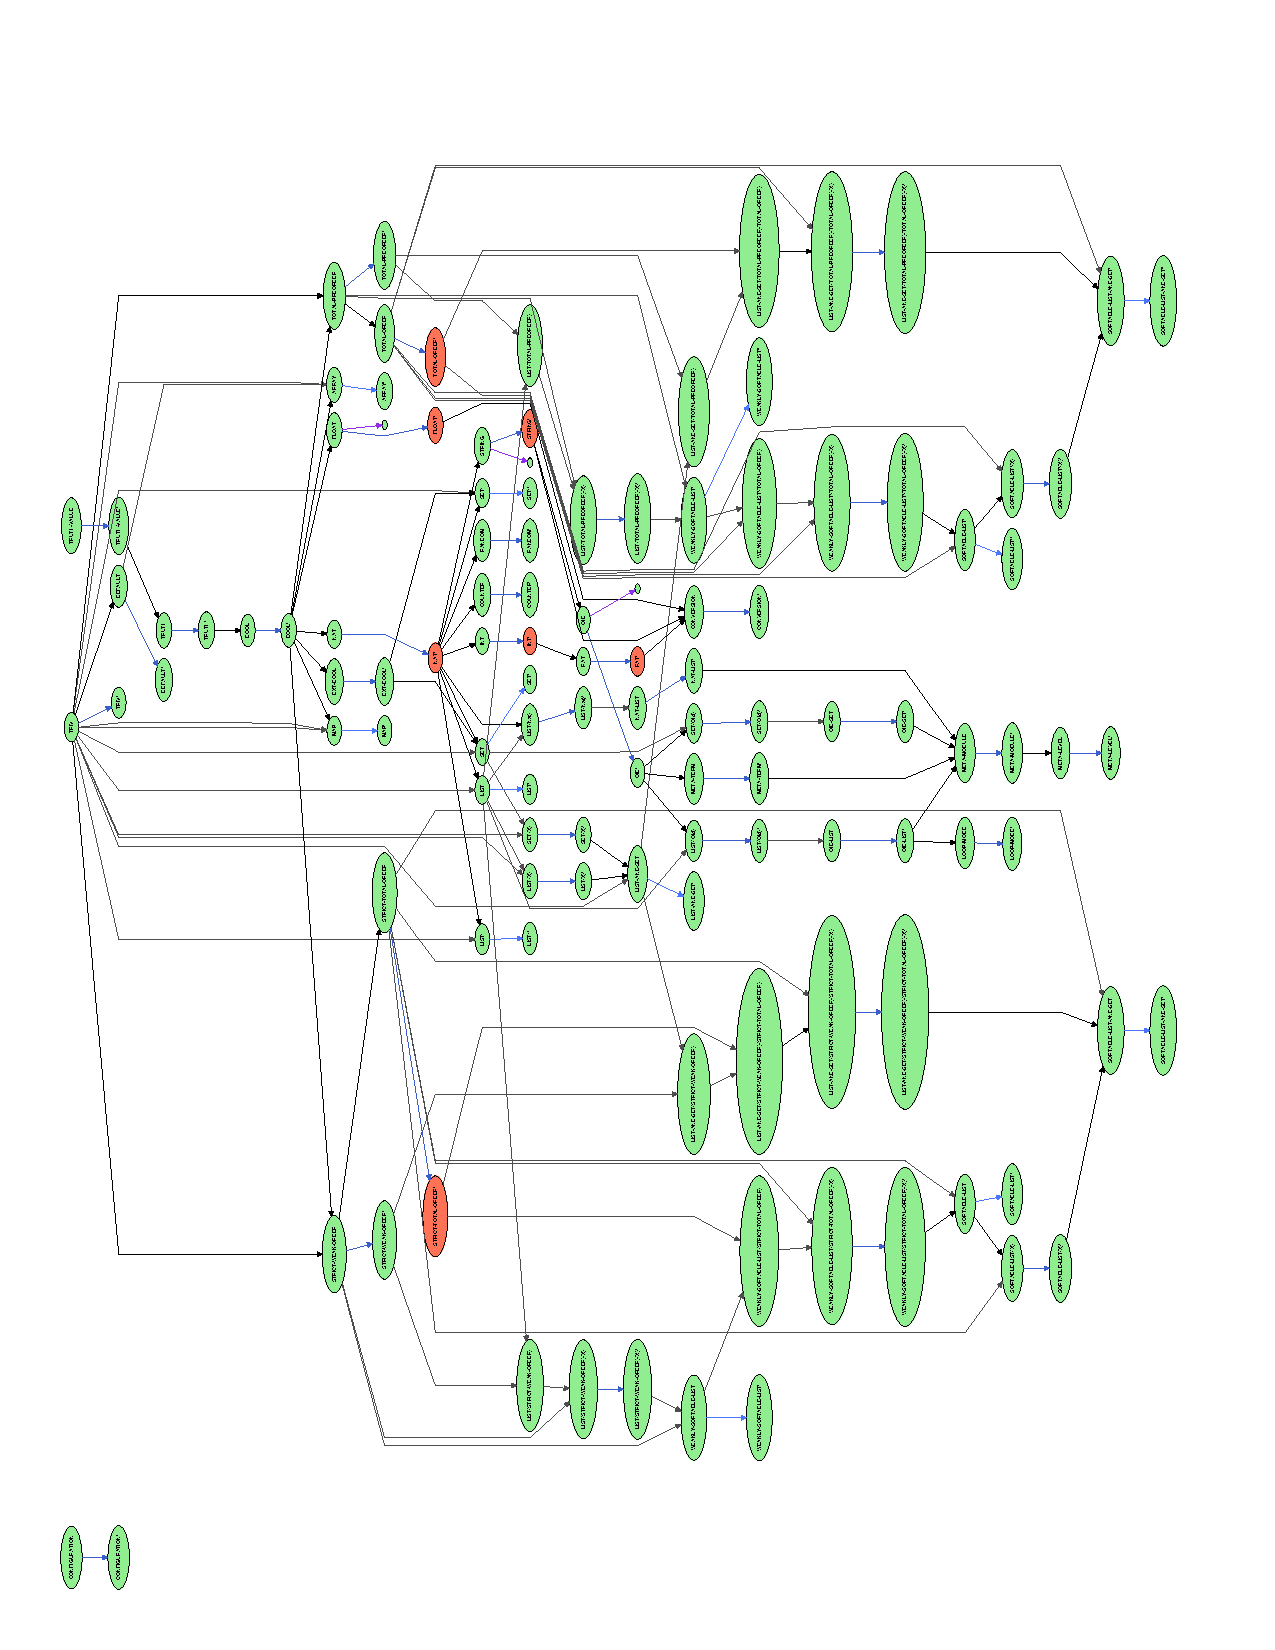
\includegraphics[width=\textwidth]{prelude-all.pdf}
  \caption{Development Graph of the Maude Prelude}\label{fig:maude-prelude-all}
\end{figure}

\begin{figure}
  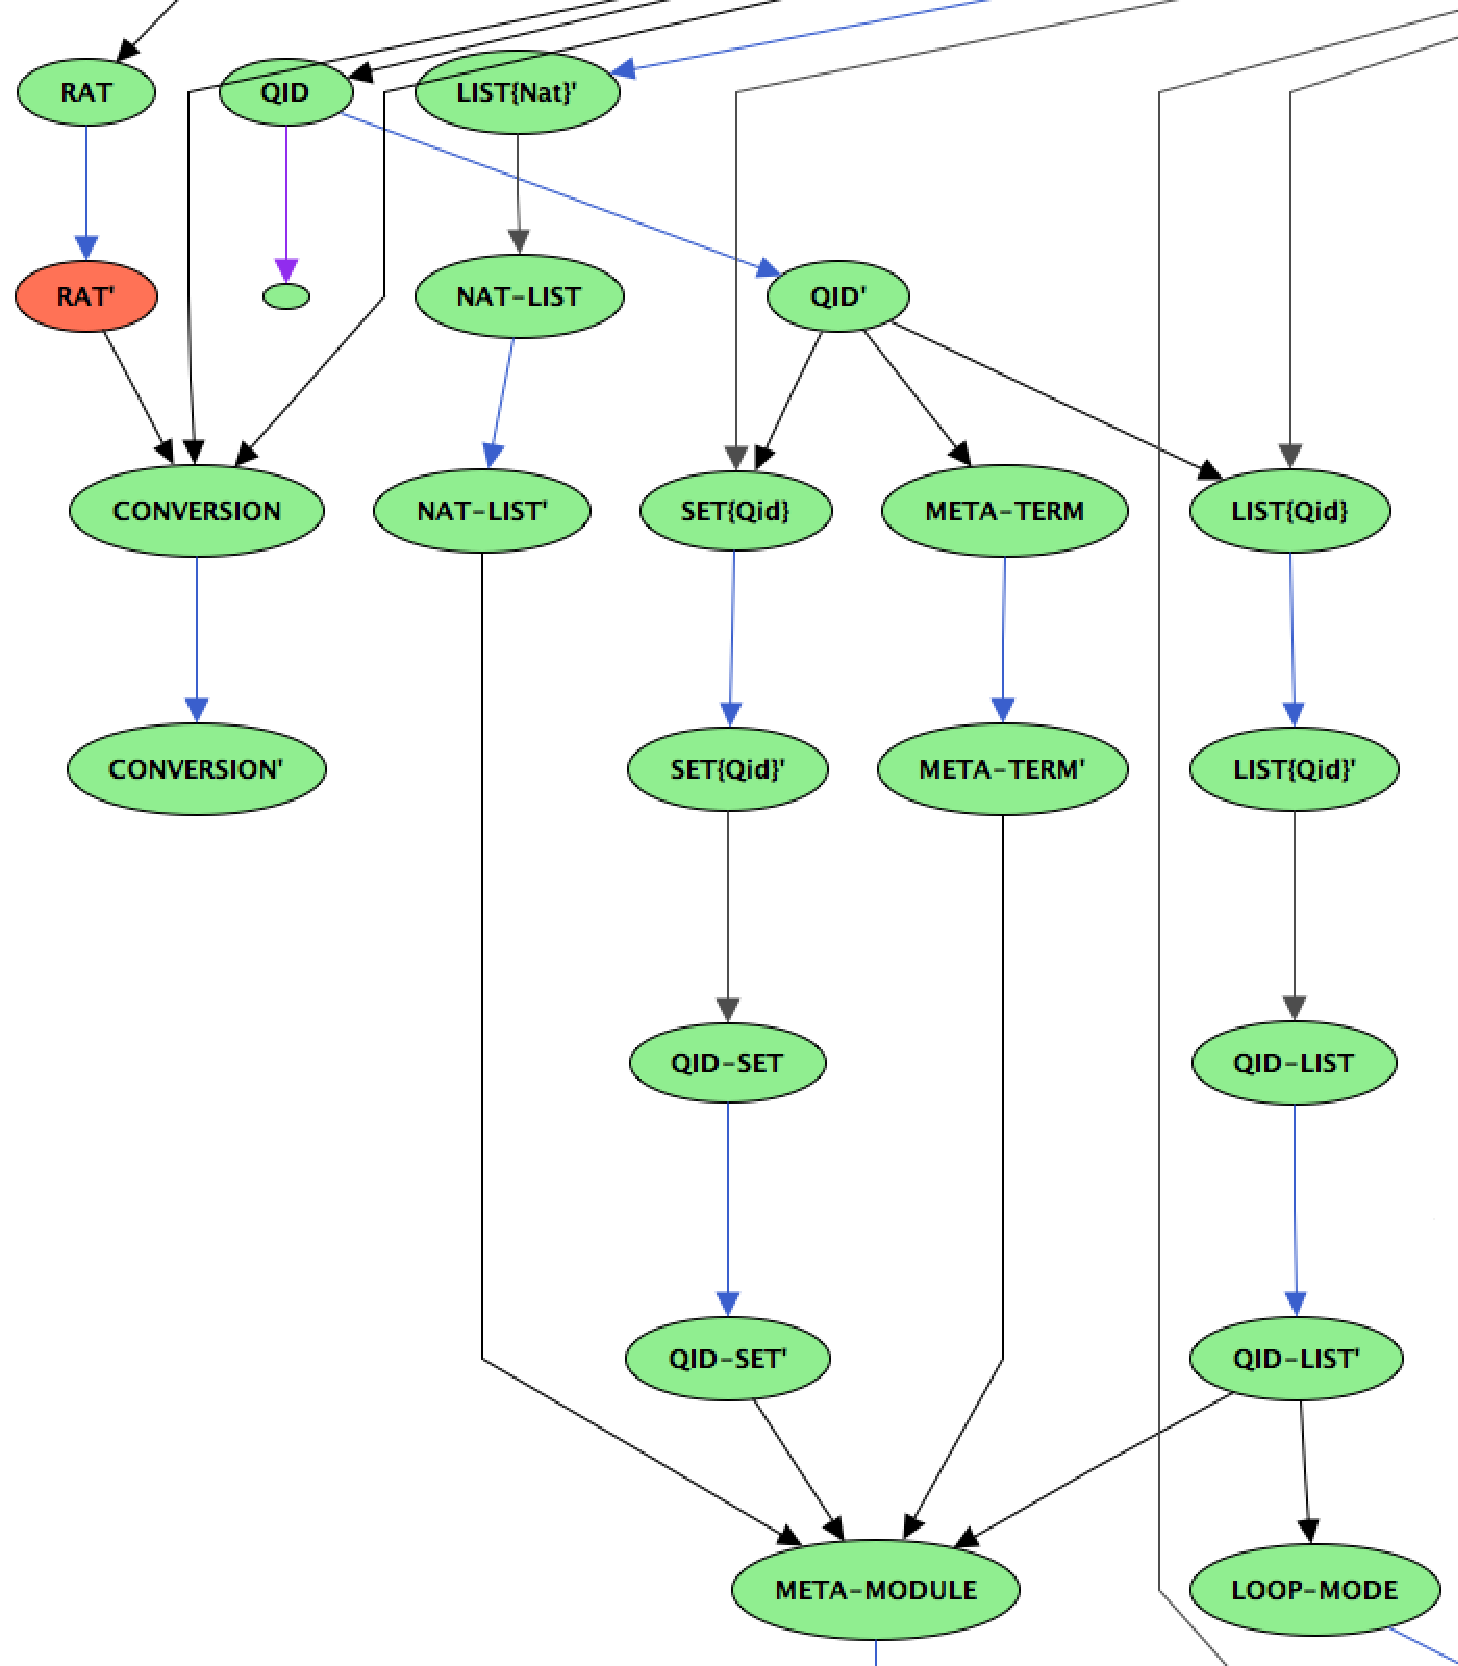
\includegraphics[width=\textwidth]{prelude-part.pdf}
  \caption{Partial Development Graph of the Maude Prelude}\label{fig:maude-prelude-part}
\end{figure}


\subsection{Translation to \Casl{}}
\label{sub:results_translation}

The logic translation can also be used to translate Maude modules to concrete syntax in other languages, like \Casl{}. Consider, as an example, the system module \textsc{Clock} and the Maude standard module \textsc{Bool}, shown in section~\ref{sub:example_clock_maude}. We can't consider them in isolation because all Maude modules \emph{include} the \textsc{Bool} module.\footnote{This default inclusion can be disabled in Maude but not yet in \Hets{}.}

The module \textsc{Clock} describes clocks in a way isomorphic to natural numbers, with an ``initial'' clock $0$ and a ``successor'' operation $t$ representing an unspecified measure of time. It then defines a rewrite rule $tick$, modelling the passage of time by advancing a clock.

The translation of the \textsc{Clock} module into a \Casl{} specification is listed in section~\ref{sub:example_clock_casl}, with one minor modification\footnote{The spec was named \textsc{Clock}; before it was anonymous.}, including the \textsc{Bool} module because of its default importation. It demonstrates nicely how rewriting and kinds are translated: Maude assigns a \emph{kind} to each connected component of the subsort relation; in the translation, they are turned into supersorts of their component. Rewriting is translated into the binary predicate $rew$, overloaded for each sort and with default rules for reflexivity and transitivity, i.e.\ axiomatised as a preorder.

We can also see how system modules and concrete rewrite rules are supported by our integration. The rule $tick$ from the \textsc{Clock} module is translated into the axiom \emph{Ax1\_16} at the end of the translated specification, establishing that $rew$ holds for each pair \mbox{$C:Clock \bullet C \times t\,C$}. Generally, a rewrite of the form $Term \Rightarrow Term' \,\mathbf{if}\, Constraint$ is translated into $Constraint \Rightarrow rew(Term, Term')$.


\subsection{Proof Goals}
\label{sub:results_proof_goals}

Maude and its syntax were designed with different principles in mind than \Casl{}, so it is only natural that some tasks common to \Hets{} or \Casl{} become clumsier when expressed in Maude.

One area where this is the case is marking propositions as proof obligations, where in \Casl{} we could use an implied extension~\cite{Mosses:2004}. To introduce proof obligations with Maude, we have to:

\begin{enumerate}
  \item Define a \emph{Module} containing our axioms.
  \item Define a \emph{Theory} holding the propositions.
  \item Introduce a \emph{View} from the theory to the module, denoting the implication that the axioms of the module entail the propositions of the theory.
\end{enumerate}

An example of this can be seen in Figure~\ref{fig:spec-maude-hom}. The specification is equivalent to the example in Figure~\ref{ex:casl-spo}, translated to Maude.

To help this situation, we can take advantage of \Hets{}'s support for \emph{structured} specifications; support for this feature by our implementation is described in section~\ref{sub:implementation_parse}. This way we can use the structuring mechanisms of \Casl{}, including implied extensions, and still write the specifications in Maude.

The structured version of this specification is displayed in Figure~\ref{fig:spec-maude-het}. The generated development graphs are of course not identical, as the pure Maude version introduces more first-class entities that appear as nodes.

\begin{figure}
  \begin{alltt}\small{}\input{SPO_PO.maude}\end{alltt}
  \caption{Specification of a Partial Order in Maude}\label{fig:spec-maude-hom}
\end{figure}

\begin{figure}
  \input{SPO_PO_Maude.pp.tex}
  \caption{Structured Specification of a Partial Order with Maude}\label{fig:spec-maude-het}
\end{figure}


\subsection{Simple Proof}
\label{sub:results_proof_simple}

The specification from Figure~\ref{fig:spec-maude-het} makes an obvious candidate for demonstrating a simple proof. Unfortunately, it doesn't work.

The problem is that in Maude the standard module \textsc{Bool} is included in every module by default, but the specification is not a pure Maude module but a structured specification using the \emph{logic} of Maude, and dependencies in structured specifications cannot currently be mixed with Maude imports.

This does not mean that proofs are unsupported though. Consider the specification of lists and their $reverse$ operation in Figure~\ref{fig:revelt-spec}. To keep this example simple, we use the very limited proof goal $\forall{E : Elt} \bullet rev(rev(E)) = E$.

\begin{figure}
  \input{RevIdemElt.pp.tex}
  \caption{Reversing a Singleton List Twice is Idempotent}\label{fig:revelt-spec}
\end{figure}

The process of proving this goal is analogous to that outlined in section~\ref{sub:introduction_hets_example}. Figures~\ref{fig:revelt-before} and~\ref{fig:revelt-after} display the development graph of the specification before and after the proof, respectively. Screenshots of the dialogues for proof tool selection and interaction with \Spass{} are displayed in Figures~\ref{fig:revelt-prove} and~\ref{fig:revelt-spass}.

\clearpage

\begin{figure}
  \begin{minipage}[b]{0.5\textwidth}
    \begin{centering}
      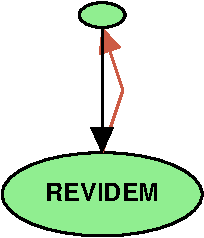
\includegraphics[width=3.5cm]{RevElt-before.pdf}
      \caption{\textsc{RevIdemElt} Proof Obligations}\label{fig:revelt-before}
    \end{centering}
  \end{minipage}
  \begin{minipage}[b]{0.5\textwidth}
    \begin{centering}
	    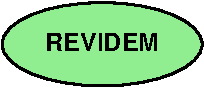
\includegraphics[width=3.5cm]{RevElt-after.pdf}
	    \caption{\textsc{RevIdemElt} Proven}\label{fig:revelt-after}
    \end{centering}
  \end{minipage}
\end{figure}

\begin{figure}
  \begin{minipage}[b]{0.5\textwidth}
    \begin{centering}
      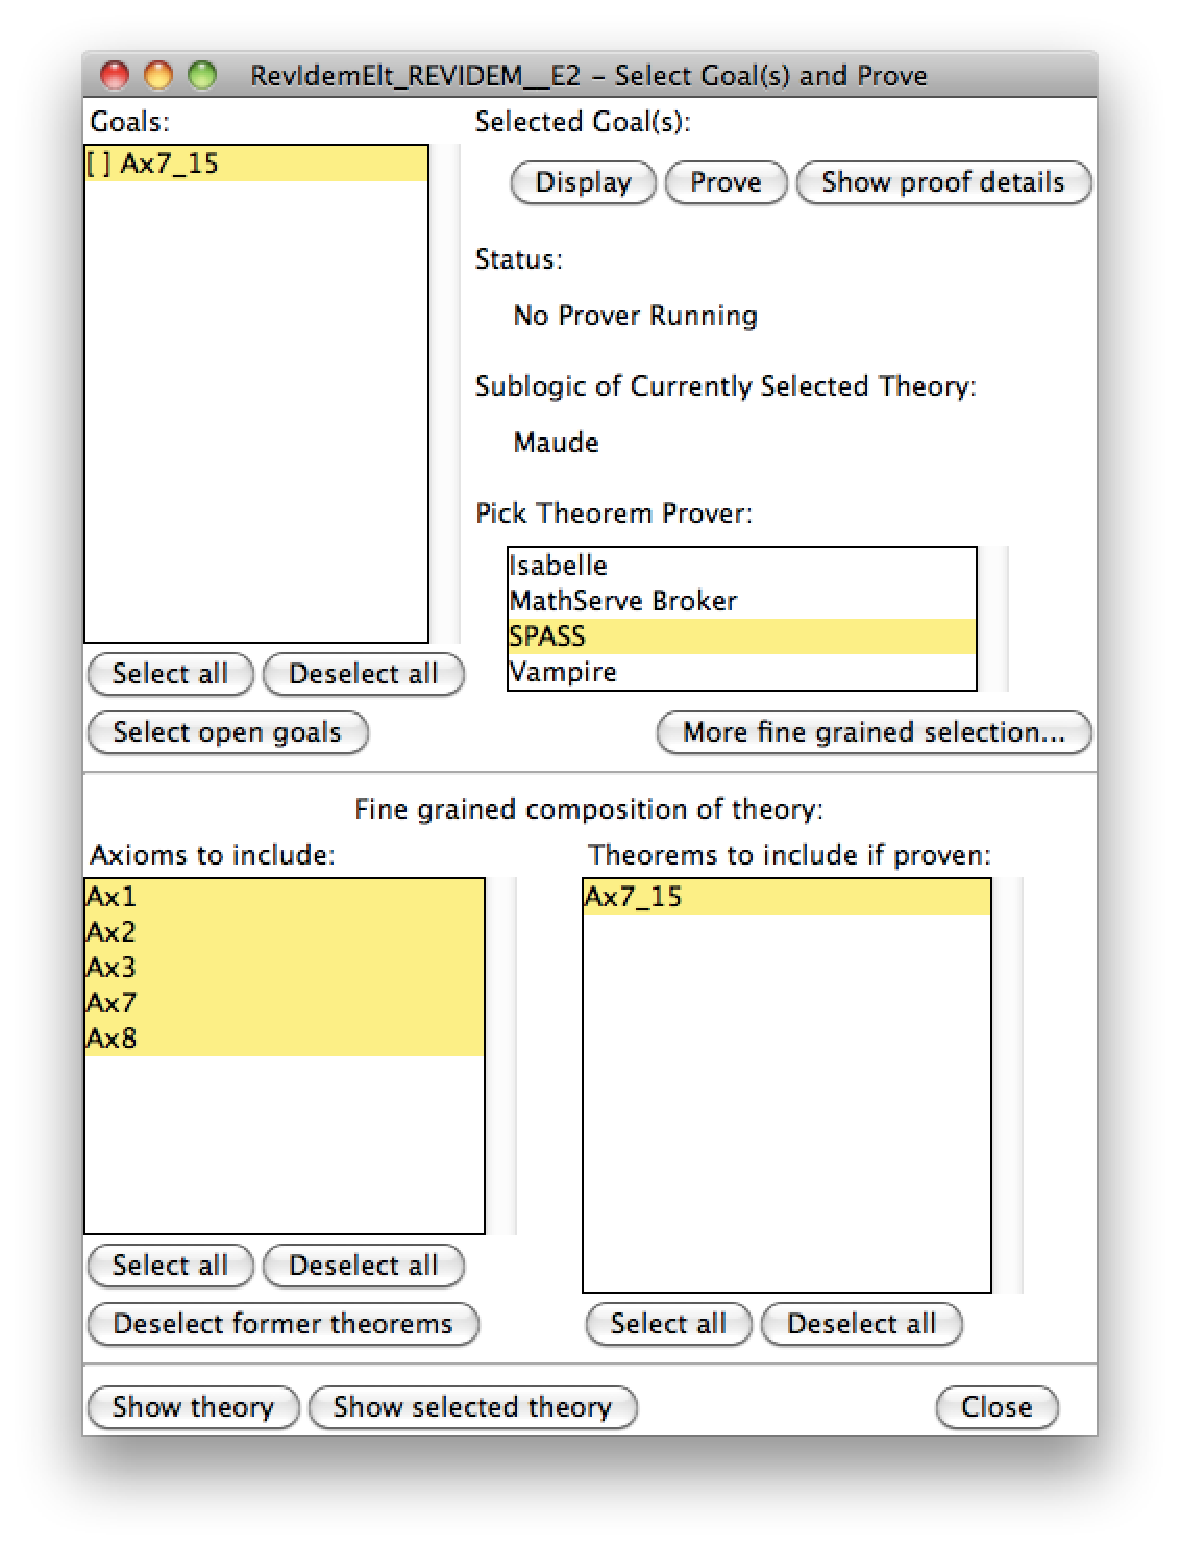
\includegraphics[width=\textwidth]{RevElt-prove.pdf}
      \caption{Proving \textsc{RevIdemElt}}\label{fig:revelt-prove}
    \end{centering}
  \end{minipage}
  \begin{minipage}[b]{0.5\textwidth}
    \begin{centering}
      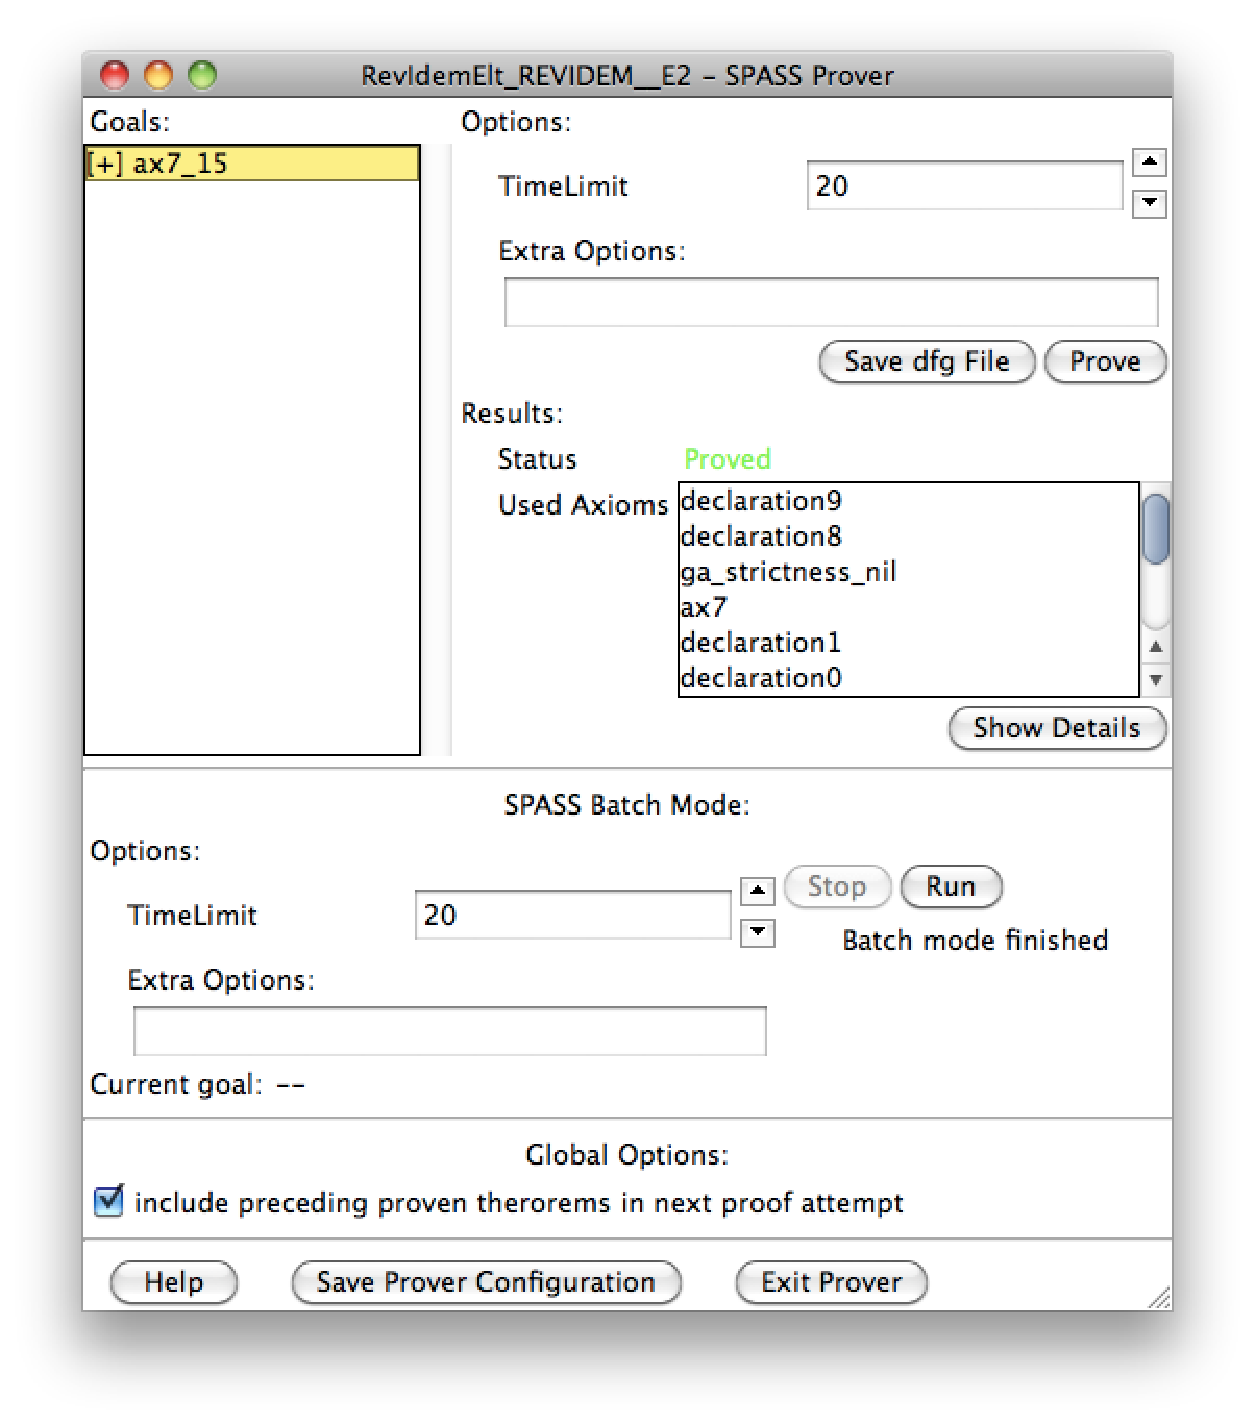
\includegraphics[width=\textwidth]{RevElt-spass.pdf}
      \caption{\textsc{RevIdemElt} Proved with \Spass{}}\label{fig:revelt-spass}
    \end{centering}
  \end{minipage}
\end{figure}

\clearpage

\subsection{Simple Proof with Rewriting}
\label{sub:sub_results_proof_rewrite}

Consider once more the \textsc{Clock} module from section~\ref{sub:example_clock_maude} and its translation in section~\ref{sub:example_clock_casl}. We can extend the translated specification as in Figure~\ref{fig:spec-clock-rewrite} to establish proof obligations on the rewriting relation, in this case firstly that the initial clock can $tick$ five times and secondly that any clock can $tick$ five times.

\begin{figure}
  \input{RewriteClock.pp.tex}
  \caption{The \textsc{Clock} Specification Extended with Proof Goals}\label{fig:spec-clock-rewrite}
\end{figure}

Notice that both the \textsc{Clock} specification we import and the sentences we extend it with are written in \Casl{}. Importing directly form Maude source files is not supported yet, and neither is the translation from \Casl{} to Maude that would be required for extending \Casl{} specifications in Maude.

The proof itself can once again be performed with \Spass{}, the screenshots for which we omit here. Figures~\ref{fig:clock-before} and~\ref{fig:clock-after} display the development graph of the specification before and after the proof, respectively.

\begin{figure}
  \begin{minipage}[b]{0.5\textwidth}
    \begin{centering}
      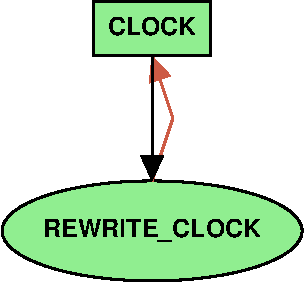
\includegraphics[width=3.5cm]{Clock-before.pdf}
      \caption{\textsc{Clock} Proof Obligations}\label{fig:clock-before}
    \end{centering}
  \end{minipage}
  \begin{minipage}[b]{0.5\textwidth}
    \begin{centering}
	    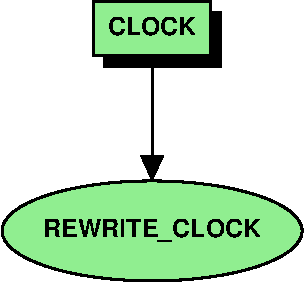
\includegraphics[width=3.5cm]{Clock-after.pdf}
	    \caption{\textsc{Clock} Proven}\label{fig:clock-after}
    \end{centering}
  \end{minipage}
\end{figure}


\subsection{Complex Proof with Isabelle}
\label{sub:results_proof_complex}

A more interesting proof than in section~\ref{sub:results_proof_simple}, involving actual induction and requiring the use of Isabelle, would be to prove the specification in Figure~\ref{fig:spec-revidem}. This proof is possible but involved and not reproduced here.

\begin{figure}[htb]
  \input{RevIdem.pp.tex}
  \caption{Reversing a List Twice is Idempotent}\label{fig:spec-revidem}
\end{figure}

Maude makes heavy use of initial and free semantics~\cite{Codescu:2010}, visible e.g.\ in the fact each Maude module generates two nodes in a development graph, the second linked to the first one with a free definition link~\cite{Mosses:2004}, but freeness cannot be handled in an institution-independent way.

A solution to this problem presented by~\cite{Codescu:2010} is to translate the models of the specification to \Casl{} and then use ``a transformation specific to the second-order extension of \Casl{} to normalise freeness.'' For details of this transformation and the proof of this specification refer to~\cite{Codescu:2010}.

% section results (end)

\clearpage
\section{Conclusion} % (fold)
\label{sec:conclusion}

\subsection{Goals of This Work}
\label{sub:conclusion_goals}

We have successfully implemented a representation of Maude as a logic in \Hets{}, with supports all of Core Maude including rewriting. This representation can be generated for both pure Maude modules and for structured specifications with parts written in Maude.

Maude modules can be incorporated into a development graph and translated into \Casl{}, and Maude can be used this way to formulate both axioms and proof goals. Maude specifications can be verified with \Hets{} using the usual set of tools, most notably \Spass{} and Isabelle.\footnote{The proofs demonstrated with \Spass{} can be replicated with Isabelle by simply applying its \emph{auto} strategy.}

Parts of the integration require additional work, particularly the issues concerning freeness alluded to in section~\ref{sub:results_proof_complex}. Freeness is also likely to be at the root of the problem mentioned at the beginning of section~\ref{sub:results_proof_simple}; the issue calls for further examination.


\subsection{Future Work}
\label{sub:conclusion_future}

The issues just mentioned are actively being worked on, including ongoing research into the problem of freeness in \Hets{}.

Other future work includes the options discussed in section~\ref{sec:analysis} but not prioritised in this work: From the side of \Hets{}, a translation from \Casl{} to Maude and the integration of Maude as a rewriting tool for \Casl{} specifications. From the side of Maude, support for the advanced features of Full Maude like object-oriented specifications.

There are also plans to relate \Hets{}' modal logic to Maude modules in order to use the Maude model checker for linear temporal logic.


\subsection{Acknowledgement}
\label{sub:conclusion_ack}

I want to thank Mihai Codescu, Till Mossakowski, Adri\'an Riesco and Christian Maeder for their work on~\cite{Codescu:2010}, which can be regarded as dual to this work, establishing the theoretical foundation for this integration, and for their contributions to the implementation.

Additional thanks to my supervisor Till Mossakowski for sharing advice, expertise and motivation, and to my personal reviewer Tobias Hametner for his persistence.

Last but not least thanks to my family and my wife Julia for their love and continued support, without which I could not have finished this thesis.

% section conclusion (end)

\appendix

\clearpage
\section{Implementation of the Maude Integration} % (fold)
\label{sec:appendix_implementation}

\subsection{Listing for Module \texttt{Maude.AS\_Maude}}
\label{imp:Maude/AS_Maude.hs}
\lstinputlisting{Maude/AS_Maude.hs}
\clearpage
\subsection{Listing for Module \texttt{Maude.Language}}
\label{imp:Maude/Language.hs}
\lstinputlisting{Maude/Language.hs}
\clearpage
\subsection{Listing for Module \texttt{Maude.Logic\_Maude}}
\label{imp:Maude/Logic_Maude.hs}
\lstinputlisting{Maude/Logic_Maude.hs}
\clearpage
% \subsection{Listing for Module \texttt{Maude.Maude2DG}}
% \label{imp:Maude/Maude2DG.hs}
% \lstinputlisting{Maude/Maude2DG.hs}
% \clearpage
\subsection{Listing for Module \texttt{Maude.Meta.AsSymbol}}
\label{imp:Maude/Meta/AsSymbol.hs}
\lstinputlisting{Maude/Meta/AsSymbol.hs}
\clearpage
\subsection{Listing for Module \texttt{Maude.Meta.HasLabels}}
\label{imp:Maude/Meta/HasLabels.hs}
\lstinputlisting{Maude/Meta/HasLabels.hs}
\clearpage
\subsection{Listing for Module \texttt{Maude.Meta.HasName}}
\label{imp:Maude/Meta/HasName.hs}
\lstinputlisting{Maude/Meta/HasName.hs}
\clearpage
\subsection{Listing for Module \texttt{Maude.Meta.HasOps}}
\label{imp:Maude/Meta/HasOps.hs}
\lstinputlisting{Maude/Meta/HasOps.hs}
\clearpage
\subsection{Listing for Module \texttt{Maude.Meta.HasSorts}}
\label{imp:Maude/Meta/HasSorts.hs}
\lstinputlisting{Maude/Meta/HasSorts.hs}
\clearpage
\subsection{Listing for Module \texttt{Maude.Meta}}
\label{imp:Maude/Meta.hs}
\lstinputlisting{Maude/Meta.hs}
\clearpage
\subsection{Listing for Module \texttt{Maude.Morphism}}
\label{imp:Maude/Morphism.hs}
\lstinputlisting{Maude/Morphism.hs}
\clearpage
\subsection{Listing for Module \texttt{Maude.Parse}}
\label{imp:Maude/Parse.hs}
\lstinputlisting{Maude/Parse.hs}
\clearpage
% \subsection{Listing for Module \texttt{Maude.PreComorphism}}
% \label{imp:Maude/PreComorphism.hs}
% \lstinputlisting{Maude/PreComorphism.hs}
% \clearpage
\subsection{Listing for Module \texttt{Maude.Printing}}
\label{imp:Maude/Printing.hs}
\lstinputlisting{Maude/Printing.hs}
\clearpage
\subsection{Listing for Module \texttt{Maude.Sentence}}
\label{imp:Maude/Sentence.hs}
\lstinputlisting{Maude/Sentence.hs}
\clearpage
% \subsection{Listing for Module \texttt{Maude.Shellout}}
% \label{imp:Maude/Shellout.hs}
% \lstinputlisting{Maude/Shellout.hs}
% \clearpage
\subsection{Listing for Module \texttt{Maude.Sign}}
\label{imp:Maude/Sign.hs}
\lstinputlisting{Maude/Sign.hs}
\clearpage
\subsection{Listing for Module \texttt{Maude.Symbol}}
\label{imp:Maude/Symbol.hs}
\lstinputlisting{Maude/Symbol.hs}

% section appendix_implementation (end)

\clearpage
\section{Additional Example Specifications} % (fold)
\label{sec:appendix_example}

\subsection{\textsc{Clock} and \textsc{Bool} in Maude}
\label{sub:example_clock_maude}
\begin{alltt}\small{}\input{Bool.maude}\end{alltt}
\begin{alltt}\small{}\input{Clock.maude}\end{alltt}

\subsection{\textsc{Clock} and \textsc{Bool} translated to \Casl{}}
\label{sub:example_clock_casl}
\input{Clock.pp.tex}

% section appendix_example (end)

\clearpage
\thispagestyle{plain}
\listoffigures

\clearpage
\pagestyle{plain}
\bibliographystyle{acm}
\bibliography{maude}

\end{document}
